\chapter{微积分 - 梯度-积分}

\begin{figure}[ht]
  \centering
  \includegraphics[width=1\textwidth]{asset/茶桁的 AI 秘籍_Math_12.png}
\end{figure}

\newpage

上一节课, 我们讲了方向导数, 并且在最后留了个小尾巴, 是什么呢? 就是梯度. 

我们再来回看一下这个式子:
\begin{align*}
  \begin{bmatrix} f_x \quad f_y  \end{bmatrix}
  \begin{bmatrix} cos \alpha \\ cos \beta \end{bmatrix}
\end{align*}
之前提到过, 梯度的方向是函数变化最快的方向. 因为\textit{任何方向, 只有和梯度保持同向的时候, 方向导数才最大. 所以, 梯度的方向是函数变化最快的方向}. 这是一个很重要的一个结论, 我们在人工智能, 以及神经网络的领域里面, 为什么我们用的算法都是以梯度下降为基础的? 原因就在于梯度方向是下降、上升最快的. 我们其他的方向可以不用看, 就把握住梯度就可以了. 

这个结论非常重要, 哪怕之前那些推导大家看不太懂都没有关系, 但是这句话则非常重要, 我们再拿过来重申一遍:

\textcolor{red}{当$\nabla f$和$\vec l$方向一致时,它们的内积最大,梯度的方向是函数变化最快的方向. }

大家一定要记住. 

\section{梯度}

我们该怎么样去理解\textbf{梯度的方向是函数变化最快的方向}呢? 拿地理上面的等高线去做一个比较, 如图\ref{fig:img13_1}. 

\begin{figure}[ht]
  \centering
  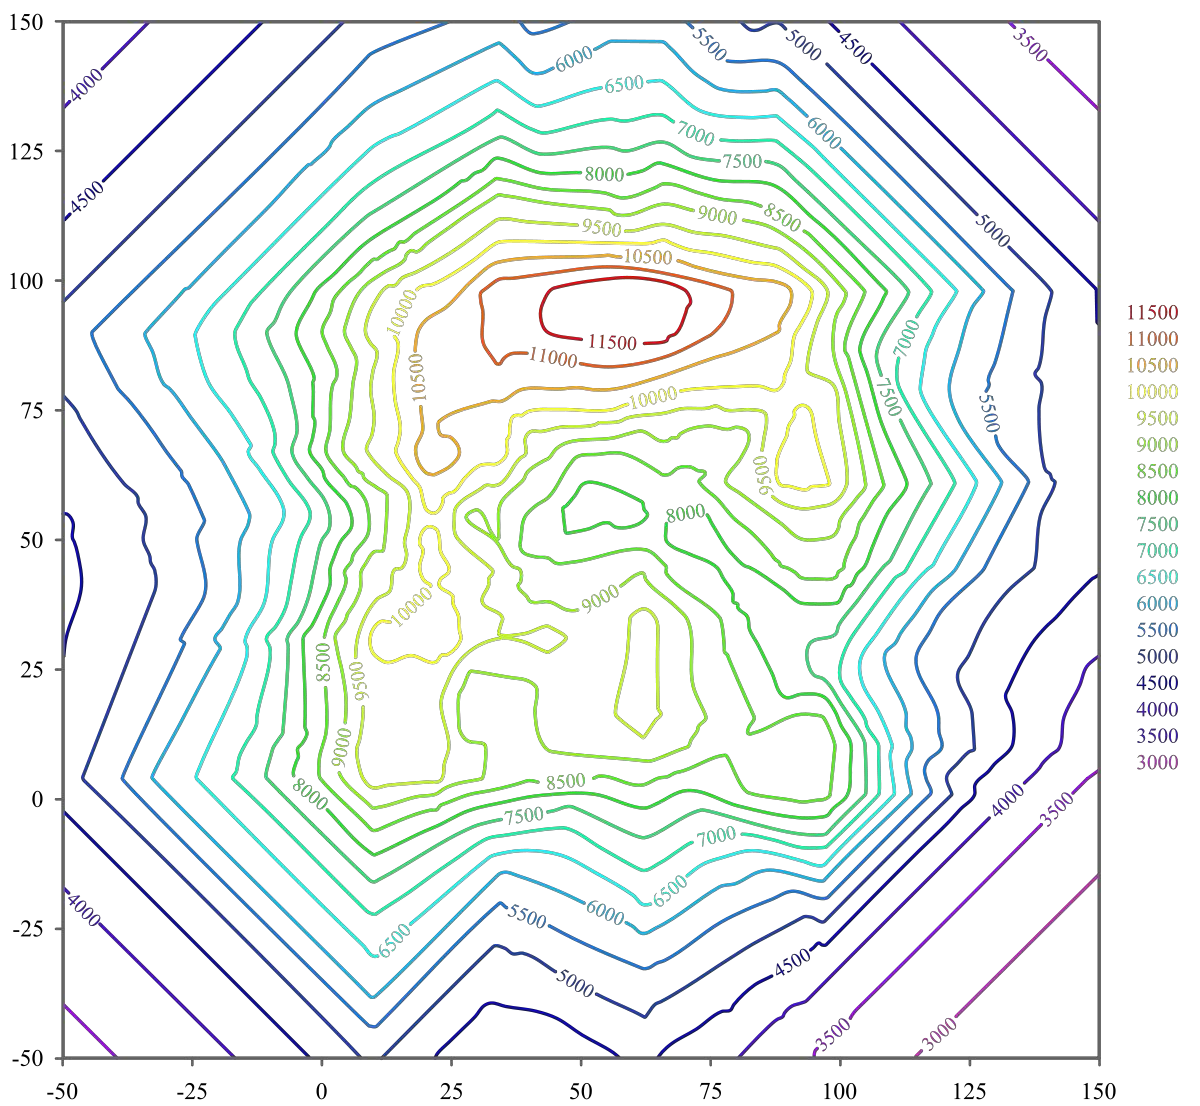
\includegraphics[width=0.45\textwidth]{asset/20230901221656.png}
  \caption{}
  \label{fig:img13_1}
\end{figure}

在初中地理上, 大家应该都学过等高线. 怎么样去看等高线? 

首先, 它同一圈表示同样的高度, 当我们沿着这条线, 和它垂直方向的时候, 我们知道我们下山最快的途径. 我们要是在山顶需要下山, 怎么样下山最快? 就是求这些线垂直的方向, 找出垂直的一条线然后再下山. 

打比方, 我们同样是走了 100 米, 图\ref{fig:img13_2}中沿着 X 方向肯定就比沿着 Y 方向下山下去的海拔要更多. 

\begin{figure}[ht]
  \centering
  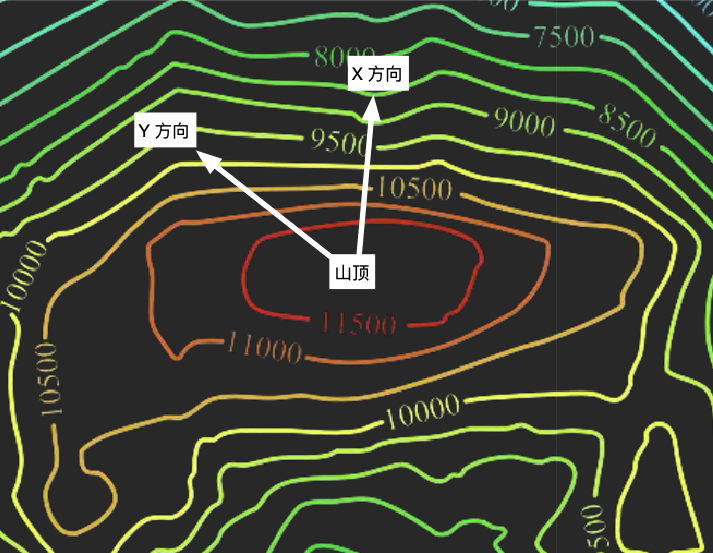
\includegraphics[width=0.5\textwidth]{asset/20230901223615.png}
  \caption{}
  \label{fig:img13_2}
\end{figure}

这其实就是因为梯度的方向是函数变化最快的方向, 这点在图里面也是一样的. 

梯度是各个方向的偏导数构成的向量, 如果函数有$x_1, x_2,..., x_n$, 这么多自变量, 各个偏导数组合在一起构成向量就叫做梯度. 
\begin{align*}
  (\frac{\partial y}{\partial x_1},\frac{\partial y}{\partial x_2},..., \frac{\partial y}{\partial x_n})
\end{align*}
梯度我们一般用倒三角的符号$\nabla$表示, 读作`nabla`, 然后再和函数写在一起,表记如下:
\begin{align*}
  \nabla f(x_1, x_2, ..., x_n)
\end{align*}
或者我们干脆写成$grad f(x_1, x_2, ..., x_n)$,  $\mathord{grad}$就是梯度的英文单词$\mathord{gradient}$的简写. 大家以后看到$\nabla$或者说$grad$, 就是表示函数的梯度. 

那人工智能里面为什么要用梯度下降算法呢?  我们刚才说过, 梯度的方向是函数变化最快方向. 除此之外其实还有一种问题, 比如说对于二次函数$y=x^2$, 直接通过初中二次函数的知识就可以求出来, 最小值就是在对称轴或者说顶点处取得. 那直接一个式子就把它写出来了, 为啥还非得这么费劲迭代? 还去设计学习率、设计补偿;每一次向极值点或者说最值点逼近多少. 

其实是因为很少有情形是可以直接求出解析解的. 什么叫做解析解呢, 就是关于$y = x^2$, 你能求出对称轴是多少、顶点坐标是什么、顶点坐标的纵坐标可能对应的最值, 这就叫做解析解. 就是通过代数的方法可以一步到位直接求出最后解, 叫做解析解. 

但是在我们现实生活当中、在工程项目里面, 尤其是神经网络所拟合的这些函数很难一下子求出解析解, 甚至有的情况你是求不出来. 所以我们需要用梯度这种方式不断的去迭代, 去逼近它.  在这里梯度所对应其实就是类似于数值解. 

刚才我们讲了解析解是可以直接计算出来的, 而数值解只能一步一步的去逼近它求得近似值. 

举一个例子, 比如说, 我们想要求函数$z=x^2+y^2$何时取到最小值, 对于这样一个实例, 其实我们很容易求解, 就是两个维度的二次函数的堆积. 我们分别求出它顶点坐标横坐标, 然后我们就能知道函数在何处取到最小值, 具体步骤如下:
\paragraph{函数 $z = f(x, y) = x^2 + y^2$ 何时取到最小值?}
\begin{align*}
  & \frac{\partial f}{\partial x} = 2x, \quad \mbox{令}\frac{\partial f}{\partial x} = 0 \to x = 0\\
  & \frac{\partial f}{\partial y} = 2y, \quad \mbox{令}\frac{\partial f}{\partial y} = 0 \to y = 0 \\
  & \mbox{当}x=0, y=0\mbox{时函数取到最小值}
\end{align*}

来看图\ref{fig:img13_3}, 这张图大家可以看到, 四周都是高高的, 中间是低洼, 凹进去了. 在这种情况下, 很容易一眼就知道肯定中心处是最小值. 

\begin{figure}[ht]
  \centering
  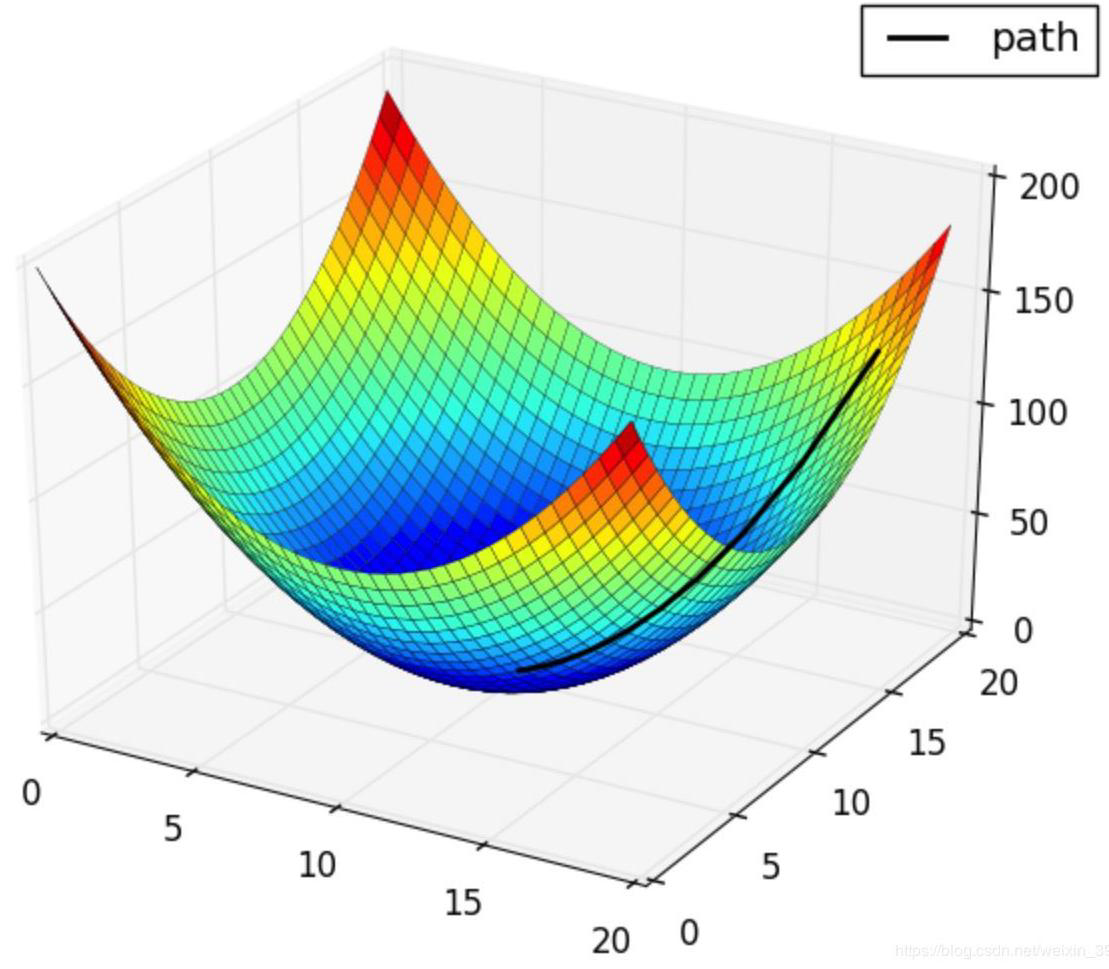
\includegraphics[width=0.5\textwidth]{asset/20230902170354.png}
  \caption{}
  \label{fig:img13_3}
\end{figure}

再来看图\ref{fig:img13_4}, 对于现在这张图中的函数想要从初始点一路到箭头终点想要求出一个解析解, 其实是比较困难的一件事情. 而且, 还有可能遇到一些其他情况, 就比如说当你以为自己求出了一些所谓的类似于二次函数的顶点.

\begin{figure}[ht]
  \begin{minipage}[t]{0.48\textwidth}
    \centering
    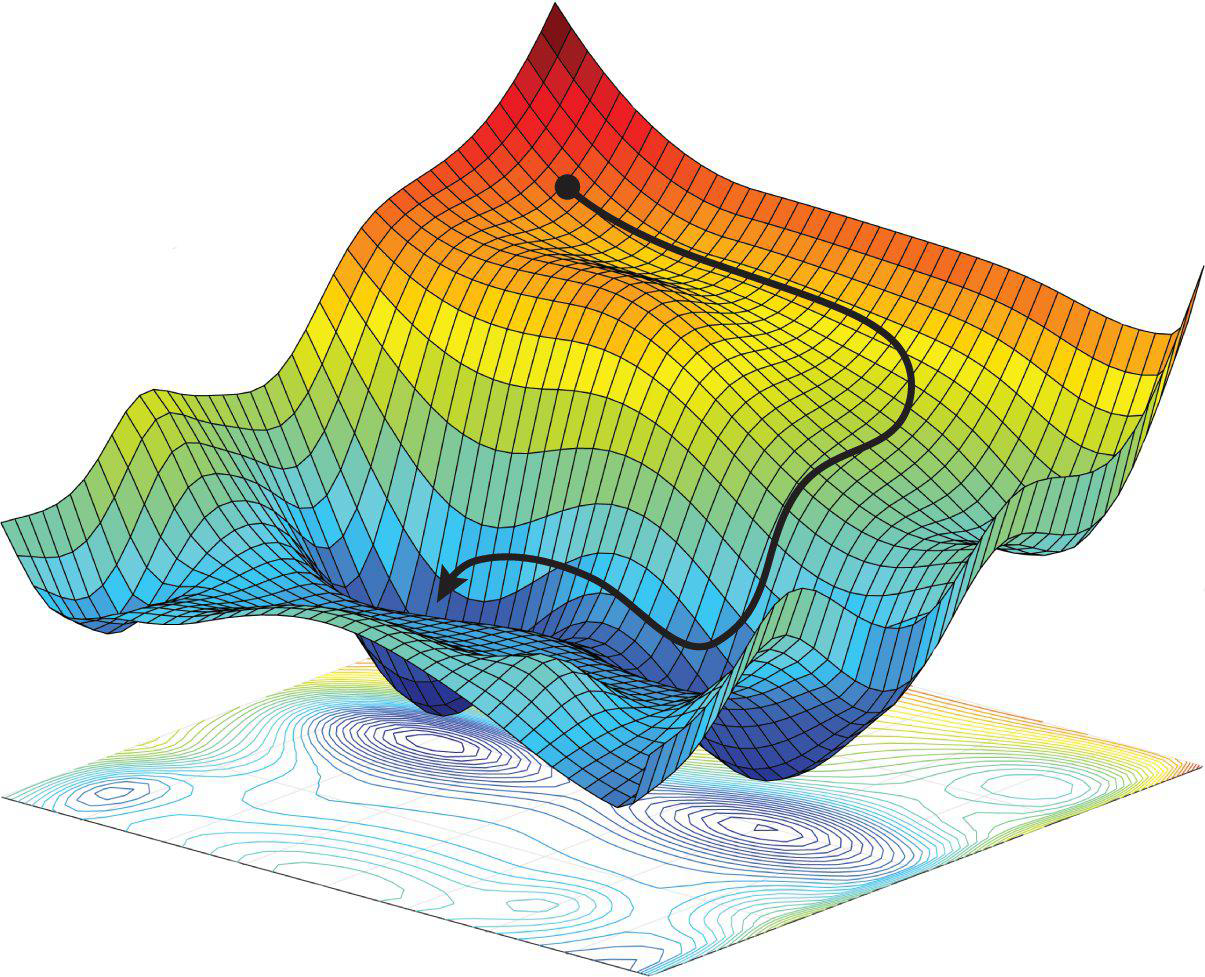
\includegraphics[width=\textwidth]{asset/20230902174547.png}
    \caption{}
    \label{fig:img13_4}
  \end{minipage} %
  \hspace{1em}
  \begin{minipage}[t]{0.48\textwidth}
    \centering
    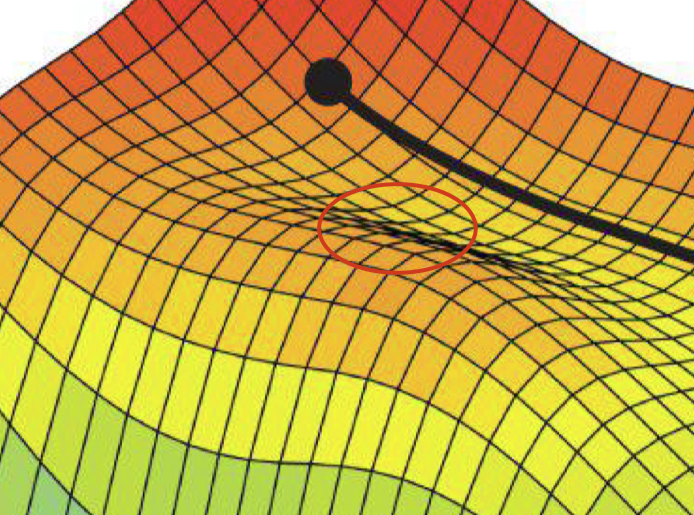
\includegraphics[width=\textwidth]{asset/20230902174840.png}
    \caption{}
    \label{fig:img13_5}
  \end{minipage}
\end{figure}

如图\ref{fig:img13_5}, 假如我们在标示的地方有得这么一个点.它的变化趋于平缓, 这是局部极小值点. 你在这里的时候以为求到了, 但其实它不是最值点, 那这个解析解也就白搭了. 或者虽然它在所在的那个区域变化平缓, 但是其实并不是一个最值点, 往下还有一个凹下去的下坡, 往左上则是往上增长的一个趋势, 这种点呢叫做鞍点. 其特点是沿着某一方向是稳定的, 另一条方向是不稳定的奇点. 还有一个概念:驻点, 也是差不多类似的这么一个意思. 

所以对于这种比较复杂的函数而言, 对于它就没办法求到解析解, 只能一步一步逼近. 在逼近的时候, 我们也有一些办法去规避掉这些东西. 比如说, 梯度可能遇到极小值问题, 同时它还有鞍点、驻点这些问题咋办? 没办法了, 我们如果是用解析解的话就白瞎了. 但如果是数值解, 梯度下降我们就可以通过设置每一步下降多少, 可以通过调节学习率(步长)来解决. 

又或者, 初始化方法. 比如最初始的点放在哪里, 可以是图中任意一个地方, 多个位置都去尝试一下的话就有很大的把握去规避掉这些问题. 

所以, 这也是梯度为什么在人工智能发展到现在依然是核心基石的一个原因. 

接着我们来看一个动图展示\ref{fig:img13_6}

\begin{figure}
  \centering
  \includegraphics[width=0.5\textwidth]{asset/截屏 2023-12-31 16.01.00.png}
  \caption{动图无法正确显示, 点击\href{https://raw.githubusercontent.com/hivandu/notes/main/img/20230902191105.gif}{查看原图}}
  \label{fig:img13_6}
\end{figure}

对于这种二次函数而言, 设置学习率等于 0.2,梯度为:$(\frac{\partial z}{\partial x}, \frac{\partial z}{\partial y})$, 那具体的每一步是怎么迭代的呢? 

打比方说图中的起始点为$x, y$, 之后先求一下梯度, 然后令上一步的$x$,  减去学习率(每步跨多长的步长)乘上梯度, 一点一点的这样迭代. 因为梯度本身是对应着增长的方向, 那么弄个减号, 梯度就对应着下降的方向. 

所以 x 减去学习率乘上梯度, 其实就朝着最小值的方向跑了. 学习率控制每一步跑多少. 完整式子如下:

\paragraph{多元函数: $z = x^2 + y ^2$, 学习率: $\eta = 0.2$, 梯度: $(\frac{\partial z}{\partial x}, \frac{\partial z}{\partial y})$}
\paragraph{迭代}:
\begin{align*}
  & x = x - \eta \cdot \frac{\partial z}{\partial x} \\
  & y = y - \eta \cdot \frac {\partial z}{\partial y}
\end{align*}

说个题外话, 有没有人想过为什么我们总是要求最小值, 而很少要求最大值? 虽然人工智能的一些场景里是要求最大值的, 但是最大值在计算方面不太好去做, 会面临数值溢出的问题, 所以我们一般都是求最小值. 

\section{积分}

接着, 我们来看一个新的概念:积分. 

积分大部分小伙伴应该都听过, 有些人已经也学过, 我在这里给大家一步一步看一下积分是怎么来的. 

首先我们来画一个图:

\begin{python}
import numpy as np
import matplotlib.pyplot as plt
from IPython import display

x_temp = np.linspace(1, 8, 1000)
y_temp = 2*x_temp + 3

%matplotlib inline

plt.plot(x_temp, y_temp)
plt.xlim(0, 11)
plt.show()
\end{python}

我们画了这样一个直线\ref{fig:img13_7}, 大家应该都能看出来, 这是一个一次函数. 然后我们让它从 x 轴 1 点到 6 点为边, 再画垂线向上交于这条函数直线, 这样我们就围成了一个梯形, 如图\ref{fig:img13_8}.

\begin{figure}[ht]
  \begin{minipage}[h]{0.49\textwidth}
    \centering
    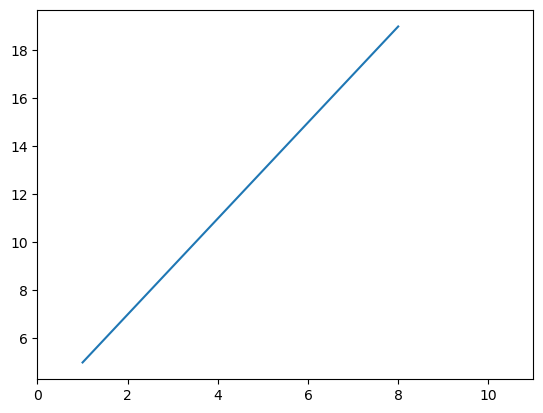
\includegraphics[width=\textwidth]{asset/20230902194132.png}
    \caption{}
    \label{fig:img13_7}
  \end{minipage} %
  \begin{minipage}[h]{0.49\textwidth}
    \centering
    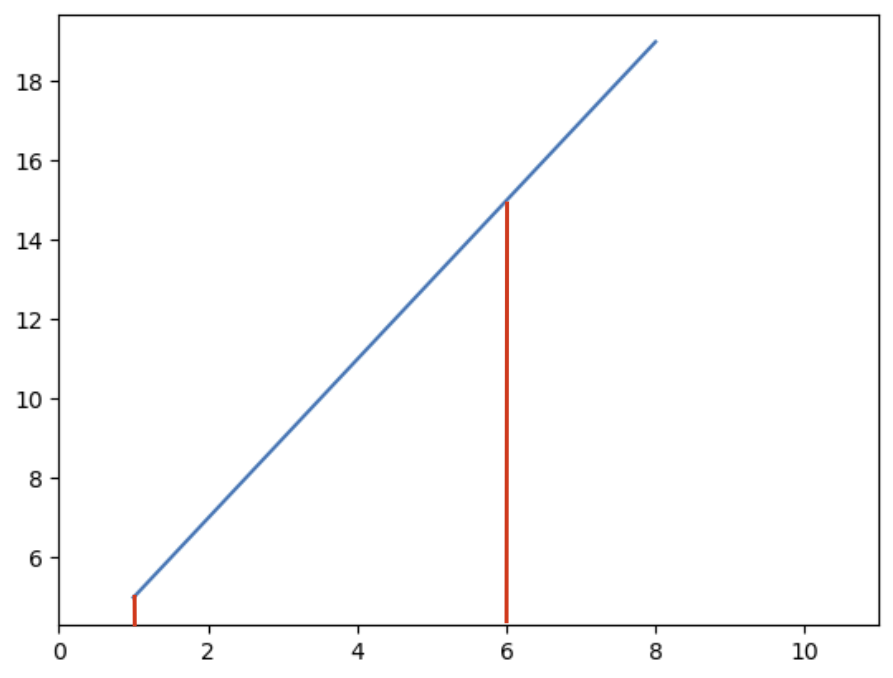
\includegraphics[width=\textwidth]{asset/20230902194557.png}
    \caption{}
    \label{fig:img13_8}
  \end{minipage}
\end{figure}

现在我们想要求这个梯形的面积应该怎么求? 是不是觉得太简单了? 上底加下底乘以高除以 2, 小学的内容还有啥好讲的? 来, 我们写一段程序, 不止是$(1, 6)$的点, 任意点我们都可求出来:

\begin{python}
# 求梯形面积
def reg_area(p1, p2):
    # p1, p2: 点的坐标
    if p1[0] < 0 or p1[1] < 0 or p2[0] < 0 or p2[1] < 0:
        print('点坐标为负值, 非法!') # 若点的坐标有负值, 则不可计算
        return -1
    height = abs(p2[0] - p1[0]) # 求梯形的高
    l1 = p1[1] # 求一个底的长
    l2 = p2[1] # 求一个底的长
    area = (l1 + l2) * height / 2
    return area

def f1(x):
    return 2*x+3

x1 = float(input('请输入第一个点的横坐标值:'))
x2 = float(input('请输入第二个点的横坐标值:'))
y1 = f1(x1)
y2 = f1(x2)

area = reg_area((x1, y1), (x2, y2))

print('此梯形的面积为:', area)
\end{python}

当我们输入(1, 6)的时候, 求得的面积为 50. 这段代码并不困难, 究其原因是因为我们已经知道公式了, 所以写起来非常简单. 大家也可以去验算一下. 

其实我想说的是, 对于规则图形, 我们都知道要怎么样去求面积. 但是问题在于对不知道面积公式的图形. 我们来尝试画一个抛物线:

\begin{python}
def f(x):
    return x**2+4

x1 = float(input("请输入第一个点的横坐标值:"))
x2 = float(input("请输入第二个点的横坐标值:"))
y1 = f(x1)
y2 = f(x2)

x_temp = np.linspace(x1, x2, 1000)
y_temp = f(x_temp)
plt.plot(x_temp, y_temp)
plt.show()
%matplotlib inline
\end{python}

然后我们输入坐标值$(-5,6)$, 得到抛物线图形\ref{fig:img13_9}:

\begin{figure}[ht]
  \centering
  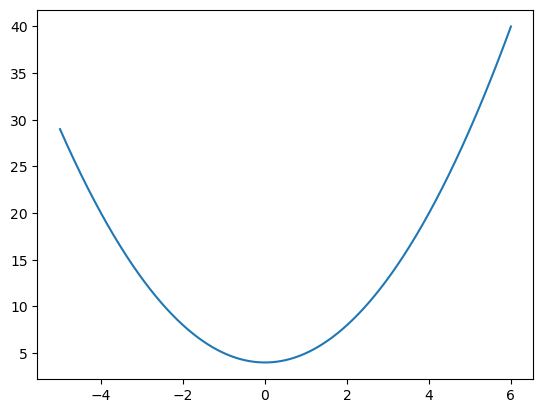
\includegraphics[width=0.6\textwidth]{asset/20230903151121.png}
  \caption{}
  \label{fig:img13_9}
\end{figure}

现在问题就在于, 我们无法直接得到这段抛物线的面积. 我们之前那个直线函数得到面积是求解它的矩形面积, 那么对于这样一个图像我们该怎么求呢? 我们找不到面积公式相关的这么一个联系, 也没人教过我们这样的二次函数怎么样去求. 

但是有另外一个办法, 就是我们可以求一个近似值, 现在从-5 到 6,  横坐标按整数分可以分成 11 份, 那我们可以将这个抛物线分成 11 份, 每一份就都是由近视的小矩形组成, 我们再把这些小矩形加在一起, 面积会近似于这个抛物线和 x 轴围成的面积. 可是我们知道, 就算是如此, 近似毕竟只是近似, 矩形是一条直线, 所以它肯定会有误差. 可是如果我们继续细分下去, 是不是它就会越来越趋近于正确的那个值? 

我们来看一个动画演示, 如图\ref{fig:img13_10}. 这个演示基本的概念就是这样, 我们可以不断用这些矩形的去拟合这个图像, 然后把这些矩形的面积加在一起. 最终就会接近于函数图像围成的面积, 当我们矩形分的非常细非常细的时候, 它就会非常逼近. 

\begin{figure}[ht]
  \centering
  \includegraphics[width=0.5\textwidth]{asset/截屏 2023-12-31 16.27.12.png}
  \caption{动图无法正确显示, 点击\href{https://raw.githubusercontent.com/hivandu/notes/main/img/20230903155234.gif}{查看原图}}
  \label{fig:img13_10}
\end{figure}



再回到我们之前的那个抛物线的图\ref{fig:img13_11}:

\begin{figure}[ht]
  \centering
  \caption{}
  \label{fig:img13_11}
  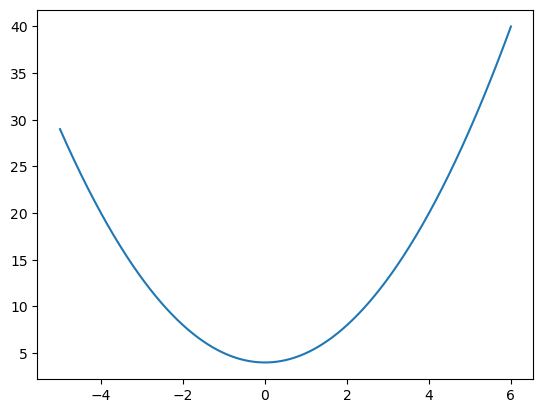
\includegraphics[width=0.5\textwidth]{asset/20230903151121.png}
\end{figure}

-5 到 6 这么一截围成的面积怎么求呢? 也是通过刚才动图里面说演示的, 用矩形组合在一起的方式给它分割. 我们在这里用一个很简单的代码去给它求一下:

\begin{python}
def irr_area(x1, x2, intervals = 1000):
    if x1 <= x2:
        x_left = x1
        x_right = x2
    else:
        x_left = x2
        x_right = x1
    dx = (x_right-x_left)/intervals
    area = 0
    x_temp = x_left
    for i in range(intervals):
        area_temp = dx * (x_temp**2+4)
        area += area_temp
        x_temp += dx
    return area
  
 for i in range(40):
    area = irr_area(-5, 6, 500*(i+1))
    print("此函数图像在这两点与横坐标轴之间围成的图形面积近似为:", area)
\end{python}

然后我们来看一下输出结果:

\begin{python}
此函数图像在这两点与横坐标轴之间围成的图形面积近似为: 157.54655399999953
此函数图像在这两点与横坐标轴之间围成的图形面积近似为: 157.60638850000103
...
此函数图像在这两点与横坐标轴之间围成的图形面积近似为: 157.66364222124224
\end{python}

我们将看到 40 个输出结果. 这些输出代表了越往下这些输出切的矩形越来越小, 分的越来越细. 直观上的感受, 分的越细对于它拟合效果更好, 就像动画演示中的一样. 如果我们切的很大, 误差就会很大, 矩形和抛物线之间会空出很大的空间. 但如果我们分的矩形越来越小, 误差就非常非常的小. 

道理就是这样, 所以我们是越往下, 分的越细. 可以看到一开始 157.54, 然后一点一点的增加, 直到它非常趋近于某一个值比较稳定了. 当然还可以继续做下去, 这里只让它做了 40 次, 其实还可以再继续往下分. 继续往下分, 就得到更精确的结果. 

对于理解积分就是通过这种方式, 我记得教科书上面其实一开始带我们理解积分的概念也是通过切割矩形. 然后把矩形之和叠加在一起, 逼近围成面积的方法来告诉我们积分的概念. 

在这里, 同样的我采取一个类似的方式带大家回忆一下. 当横坐标矩形的宽切的越来越细的时候, 矩形块的面积之和, 它和曲线围成的面积之间的误差就越来越小. 我们就可以认为, 当你每一个矩形的宽用$\Delta x$来表示, 趋向于 0 的时候($\Delta x \to 0$), 它的误差可以认为是无限逼近于 0, 就是我们极限里面的概念. 当我们用矩形的面积之和来代替围成面积的时候, 矩形面积之和就表示为:$f(x) \cdot \Delta x$ . 

在这里$\Delta x$就是每一个矩形,我在这里是假设每一个矩形都切成同样的宽. 它们的高度我们假设取了矩形左端点的函数值, 演示里其实是取了矩形中间端点的值, 我们也可以取左端点, 道理都是一样, 都是用$f(x)$表示. $f(x)\cdot \Delta x$就是每一个矩形的面积. 当我们$x$取值范围从 a 到 b 的时候,我们就把这些所有矩形的面积给它加在了一起, 符号呢叫做求和符号($\sum$), 英文叫做$\mathord{Sigma}$. 

当$\Delta x$ 无限趋向于 0 的时候, 那我们就得到了$\int$, 读作$\mathord{int}$. 我们挂上$a,b$, 就变成$\int_a^b$, 后面在跟上$f(x)dx$. $dx$ 就代表 $x$ 的增量非常小, 也就是$\Delta$趋向于 0 的时候, 我们就用 $dx$ 来表示. 这个$\int_a^b f(x)dx$, 也就是我们所说的积分. 

最后的式子如下:

\begin{align*}
  \sum_x^b = _a f(x) \cdot \Delta x => \int_a^b f(x)dx
\end{align*}

我们再继续, 在闭区间[a, b]上若不同的取样方法获得的黎曼和($\sum_x^b = f(x)\Delta x$)最终都趋于同样的极限, 则称该极限为\textit{黎曼积分}: ($\int _a^b f(x)dx$). 

那什么叫做不同的取样方法? 就是这里的这些矩形形状是怎么样的, 我可以令他每个宽都是相等, 也可以像是刚才动画演示里一样, 是各不相等的, 都可以. 所以不同的取样方法最终获得的这些矩形的面积之和, 最终都趋于同样的一个极限的话, 那我们就把这个极限叫做黎曼积分. 

除了黎曼积分之外, 积分还有其他一些形式, 比如说广义积分, 瑕积分, 反常积分, 常义积分等等, 有兴趣的同学可以自己去了解一下, 我在这里就先只涉及黎曼积分. 

所以积分就是关于用矩形面积之和去逼近它, 然后得到极限这么一个过程. 当它的长方形的宽趋于 0 的时候, 黎曼积分就出来了. 黎曼积分就对应着曲线和坐标轴围成的面积. 

这里再说一个情况, 我们这里举的例子都是在第一象限的, 如果我曲线有一节是在$x$轴下面的, 那我们就把$x$轴上方的这部分围成的面积叫做正面积, $x$轴下方的那一部分面积叫做负面积.  

比如下图这个函数图像 \ref{fig:img13_12}:

\begin{figure}[ht]
  \centering
  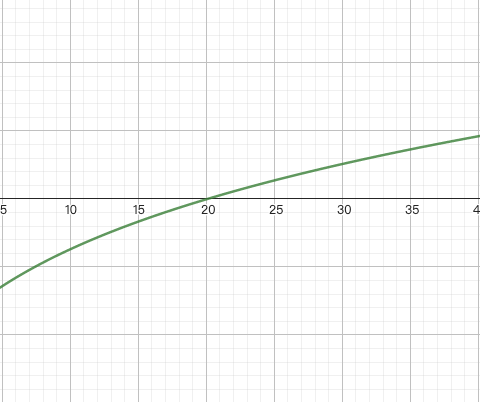
\includegraphics[width=0.5\textwidth]{asset/20230903195333.png}
  \caption{}
  \label{fig:img13_12}
\end{figure}

这个图像一部分是在$x$轴上方, 一部分在下方, 比如我们界定了(10,35)这一段, 那么我们在计算它的黎曼积分的时候, 就需要分别计算$x$轴上方的面积, 为正面积, 还有$x$轴下方的面积, 为负面积. 我们需要用正面积减去负面积. 

来看一个例子:

\begin{align*}
  \mbox{求积分}\int_1^6 2xdx\mbox{的值}
\end{align*}

积分方法是由牛顿以及莱布尼兹各自独立发现的,我们现行的使用$\int$符号是由莱布尼兹发明的, 牛顿使用的那种流数法的符号体系现在已经不用了. 继续来讲, 其中下方的 1, 表示积分的下界, 6 表示积分的上界,$2x$代表倍积函数,$dx$代表了倍积量. 

接下来, 我们来求一下积分的值. 来看这么一个例子. 

这个倍积函数的图像如图\ref{fig:img13_13}:

\begin{figure}[ht]
  \centering
  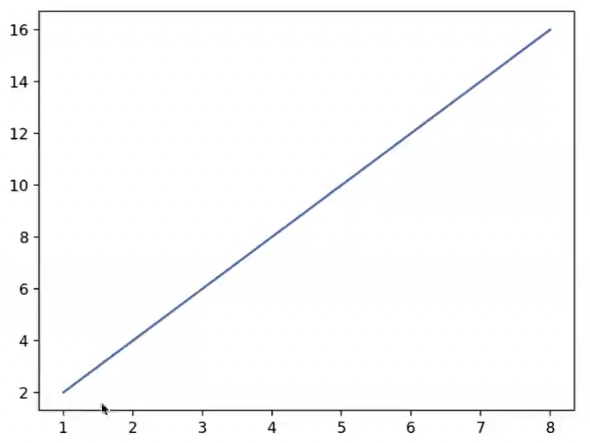
\includegraphics[width=0.5\textwidth]{asset/20230903200439.png}
  \caption{}
  \label{fig:img13_13}
\end{figure}

它就是$y=2x$,是一个正比例函数. 那我们求它的积分, 首先我们可以通过几何意义去看, 我们定义了其上届和下届的值分别为 1 和 6, 该积分对应了函数图像与$x$轴在 1 和 6 之间围成的面积, 所以这还是一个梯形,就是我们刚才做的东西. 它的积分值可以通过这种几何的方法去求解, 得到是 35. 如下:

\begin{align*}
& \int_1^6 2xdx = \frac{(2 \times 1 + 2 \times 6)\times(6-1)}{2} = 35 \\
\end{align*}

然后我们来注意一下:$x^2\vert _{x=6}-x^2 \vert _{x=1}=6^2 - 1^2 = 35$, 这段含义就是$x^2$(在$x$等于 6 的时候)减去$x^2$(当$x$等于 1 的时候). 它的结果就是 6 的平方减 1 的平方, 它也等于 35, 好神奇. 那难道说这$x^2$和$2x$之间有什么关联吗? 或者说我们把$\int_a^b2xdx$的积分写成$x^2\vert_{x=b}-x^2 \vert_{x=a}$?, 难道这两者是相等的吗? 

这里呢, 就引出了微积分里面的非常重要的一个定理了:\textbf{牛顿莱布尼兹公式}. 下一节课, 就来好好了解一下这个\textbf{牛顿莱布尼兹公式}. 